% !TeX root = RJwrapper.tex
\title{cmcR: Congruent Matching Cells Method in R for Cartridge Case
Identification}
\author{by Joseph Zemmels, Heike Hofmann, Susan VanderPlas}

\maketitle

\abstract{%
Firearm evidence identification is the process of analyzing bullets or
cartridge cases left at a crime scene to determine if they originated
from a particular firearm. Statistical methods have long been developed
and used to aid in such analyses. The Congruent Matching Cells (CMC)
method is one such method developed at the National Institute of
Standards and Technology (NIST) to quantify the similarity between two
spent cartridge cases based on the markings left by the firearm barrel
during the firing process. We introduce the first open-source
implementation of the CMC method in the R package \pkg{cmcR}. The
package will bolster forensic researchers' abilities to investigate,
validate, and improve upon current statistical methodology in the field
of forensic science.
}

\hypertarget{intro}{%
\subsection{Introduction}\label{intro}}

A \dfn{cartridge case} is a type of firearm ammunition that contains a
projectile (e.g., bullet, shots, or slug). When a firearm is discharged,
the projectile stored in the cartridge case is propelled down the barrel
of the firearm. In response, the rest of the cartridge case that remains
inside of the firearm is forced towards the back of the barrel. The
force with which the cartridge case is propelled backwards causes it to
strike the back wall, known as the \dfn{breech face}, of the barrel.
Markings due to, e.g., manufacturing imperfections are ingrained on the
breech face. When the cartridge case slams against the breech face,
these markings can be ``stamped" into either the primer of the cartridge
case or the cartridge case itself. The markings left on a cartridge case
from the firearm's breech face are called \dfn{breech face impressions}.

An example of the breech face from a 12 GAUGE, single-shot shotgun is
shown in Figure \ref{figure:barrelBF}. The hole in the center of the
breech face houses the firing pin that shoots out to strike a region on
the base of the cartridge case known as the \dfn{primer}. This in turn
ignites the propellant within the cartridge case causing a deflagration
of gases that propels the bullet forward down the barrel. Figure
\ref{figure:impressionsBF} shows a cartridge case fired from the shotgun
shown in Figure \ref{figure:barrelBF}. This cartridge case displays both
a circular impression left by the firing pin in the middle of the primer
as well as breech face impressions left on the outer region of the
primer not impressed into by the firing pin.

\begin{Schunk}
\begin{figure}[htbp]

{\centering \subfloat[\label{figure:barrelBF} Breech face of a shotgun barrel\label{fig:impressionBF1}]{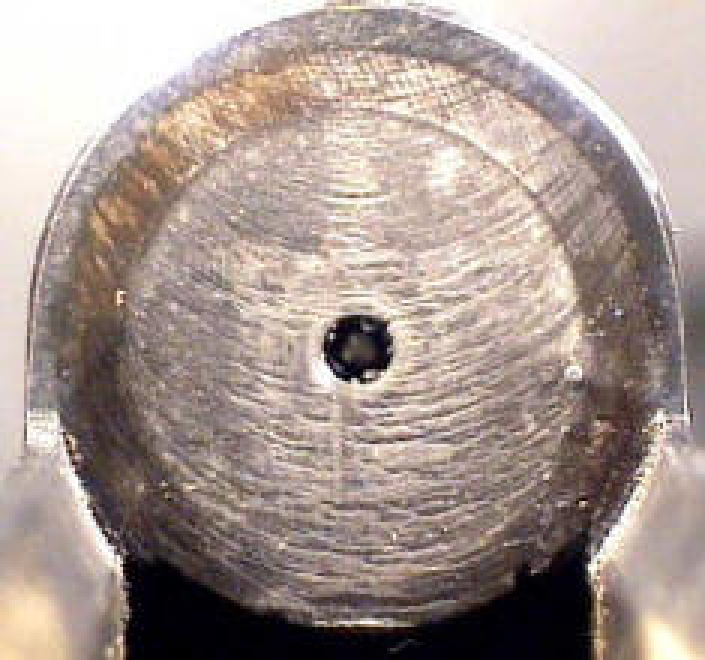
\includegraphics[width=.49\linewidth,height=2.5in]{../images/breechFace} }\subfloat[\label{figure:impressionsBF} Breech face impressions on a cartridge case primer\label{fig:impressionBF2}]{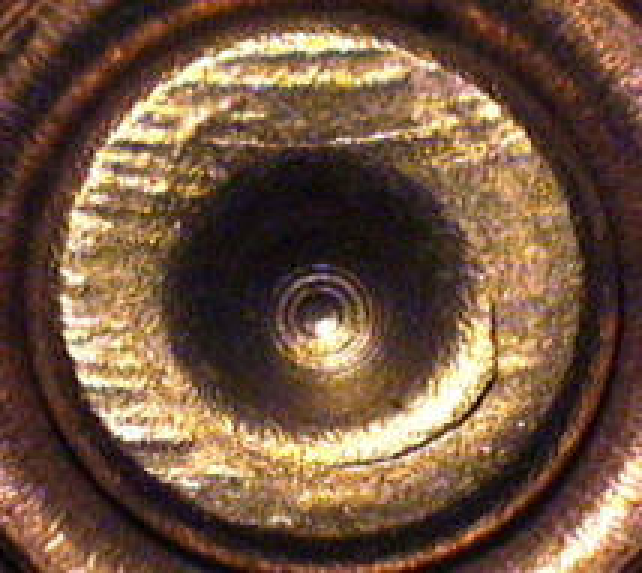
\includegraphics[width=.49\linewidth,height=2.5in]{../images/breechFaceImpression} }

}

\caption[Breech face of a barrel and breech face impression on a cartridge case \citep{doyle}]{Breech face of a barrel and breech face impression on a cartridge case \citep{doyle}}\label{fig:impressionBF}
\end{figure}
\end{Schunk}

These breech face impressions are considered to be analogous to a
firearm's ``fingerprint'' left on a cartridge case. Matching an expended
cartridge case of unknown source to one of known source based on breech
face impressions has been performed for over 100 years by forensic
practitioners \citep{firearm_id_thompson}. The development of
computational and statistical methods to perform such identification has
recently grown in interest \citep{council_strengthening_2009}.

One such method is the Congruent Matching Cells (CMC) method developed
at NIST that involves partitioning a cartridge case image or scan into a
grid of ``correlation cells" to isolate areas containing identifying
breech face impression markings \citep{song_proposed_2013}. Since its
invention in 2012, researchers at NIST have developed a number of
extensions and improvements of the CMC method. However, to date there
does not exist an openly available implementation of any of these
techniques. Rather, many methods described in the CMC literature include
a qualitative description of a proposed technique followed by results
from the authors' implementation. The description of these methods do
not delve into the intricacies of the implementation, which makes it
especially difficult to validate or assess. Additionally, some
procedures related to pre-processing the cartridge case data are
seemingly done by-hand at NIST rather than with an automated method.
This compounds the difficulty to accurately reproduce results. The
\pkg{cmcR} package provides an open-source, fully-automatic
implementation of the CMC method as originally described as well an
extension known as the ``High CMC'' method proposed by
\citet{tong_improved_2015}.

\hypertarget{data}{%
\subsection{Cartridge case data}\label{data}}

Cartridge case data commonly come in two forms: 2D grayscale images and
3D topographical scans. It is common in the CMC literature to use the 3D
topographical scans to demonstrate the efficacy of a proposed method
{[}\citep{tong_improved_2015}, \citep{chen_convergence_2017}{]}. A
variety of scans are openly available for download through the NIST
Ballistics Toolmark Research Database \citep{nbtrd}. The \pkg{cmcR}
package was designed specifically for use with the 3D topographies.

The 3D topographies are commonly stored in an .x3p (XML 3D Surface
Profile) file format that includes metainformation such as who took the
scan and the parameters under which the scan was taken (e.g., the
lateral resolution in microns). The \pkg{x3ptools} package in R provides
an interface to manipulate and visualize these .x3p files
\citep{x3ptools}. The physical surface is represented using a
\dfn{surface matrix}: a matrix of spatially-ordered elements or
``pixels" whose values correspond to the height of the cartridge case
surface at a particular location. Figure \ref{fig:cartridgeCasePair}
shows the surface matrices of a known match (KM) pair of cartridge
cases, meaning there were fired from the same firearm. Note that white
regions in the images below represent unobserved or missing values. When
read into R using the \pkg{x3ptools} package, these elements are encoded
as \code{NA}. The size of a surface matrix depends on the lateral
resolution with which the scans were taken. For example, a popular set
of scans in the CMC literature were taken by
\citet{fadul_empirical_nodate}; two of which are shown is the scan shown
in Figure \ref{fig:cartridgeCasePair}. These scans were taken with a
lateral resolution of 6.25 microns per pixel. The actual surface
matrices from this study vary around \(1200 \times 1200\) pixels in
size.

\begin{Schunk}
\begin{figure}[htbp]

{\centering \subfloat[\label{fig:rawBFs1}]{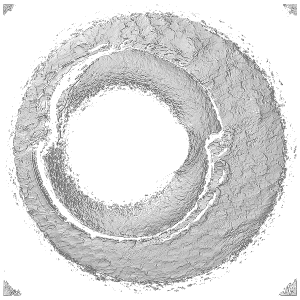
\includegraphics[width=.49\linewidth,height=.49\linewidth]{../images/fadul1-1} }\subfloat[\label{fig:rawBFs2}]{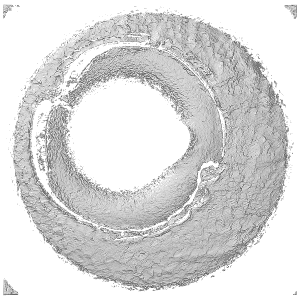
\includegraphics[width=.49\linewidth,height=.49\linewidth]{../images/fadul1-2} }

}

\caption{\label{fig:cartridgeCasePair} Two known match cartridge case scans from \citet{fadul_empirical_nodate}}\label{fig:rawBFs}
\end{figure}
\end{Schunk}

Only certain regions of a cartridge case contain identifying breech face
impression markings. \citet{song_proposed_2013} refers to these as
``valid correlation regions" that are to be used to determine whether
two cartridge cases match. The cell-based comparison procedure described
in section \protect\hyperlink{comparisonProcedure}{3.1} is designed to
emphasize such regions. However, prior to applying this procedure
cartridge scans must undergo some pre-processing to remove sections of
the cartridge case surface that do not come into contact with the breech
face of the barrel. These include a circular plateaued region in the
center of the scan that is pushed aside by the firing pin during the
firing process and clusters of observed values in the corners of the
scan that are artifacts of the staging area in which the scan was
captured. The task in pre-processing is to automatically remove these
unwanted regions from the scan to accentuate unique markings left by the
breech face. This is discussed in greater detail in section (LINK).

\hypertarget{cell-based-surface-matrix-comparisons}{%
\subsection{Cell-based surface matrix
comparisons}\label{cell-based-surface-matrix-comparisons}}

\hypertarget{comparisonProcedure}{%
\subsubsection{Cell-based comparison
procedure}\label{comparisonProcedure}}

The Congruent Matching Cells method was developed at the National
Institute of Standards and Technology to quantify the similarity between
two spent cartridge cases based on their breech face impressions. The
CMC method involves dividing a breech face impression scan into a grid
of cells and comparing each cell in one scan to a corresponding region
in the other scan. This method is motivated by the fact that breech face
markings are not uniformly impressed upon the cartridge case during the
firing process. As such, only certain sections of the cartridge case
have identifiable markings that make it possible to match to a firearm.
Calculating a similarity score between the entirety of two cartridge
case surfaces might not highlight these identifying regions. Instead,
the number of highly similar cell pairs between the two scans can be
used as a more granular similarity metric.

\begin{Schunk}
\begin{figure}[htbp]

{\centering 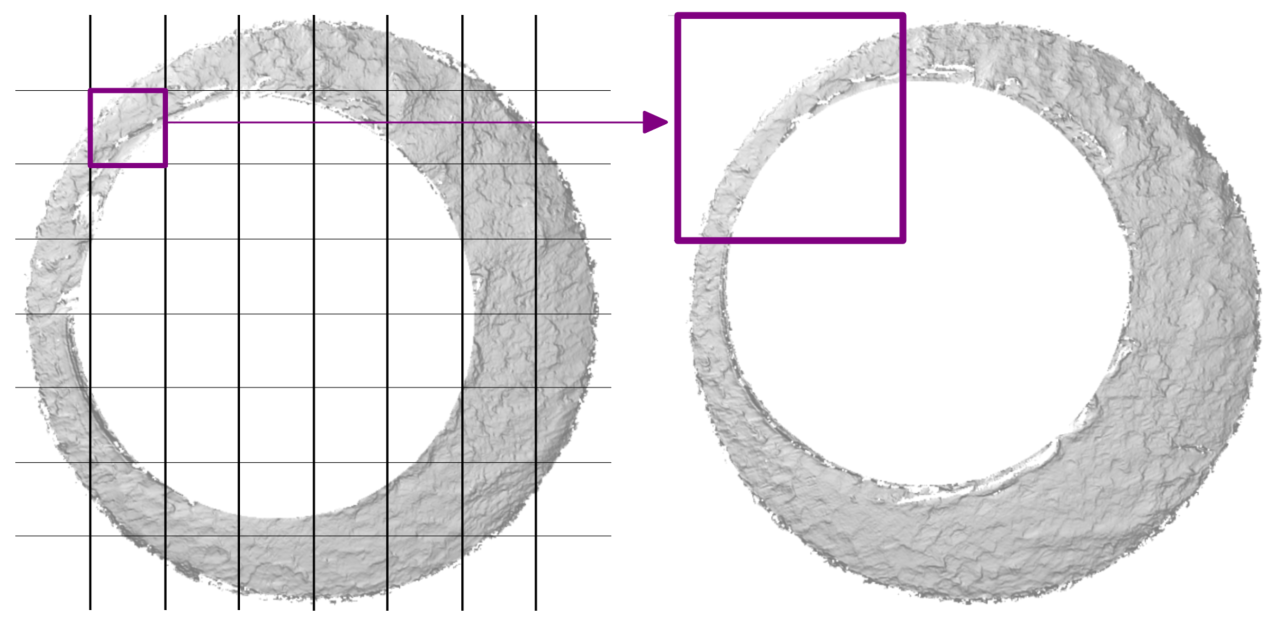
\includegraphics[width=\textwidth]{../images/cmc_illustration} 

}

\caption{\label{fig:cmc_illustration} Illustration of comparing a "cell" in one cartridge case scan to a region in another}\label{fig:unnamed-chunk-1}
\end{figure}
\end{Schunk}

Figure \ref{fig:cmc_illustration} illustrates the cell-based comparison
procedure between two cartridge case scans. The scan on the left is
divided into a grid of \(8 \times 8\) cells. Each cell is paired with an
associated larger region in the other scan. The absolute location of
each cell and region in their respective surface matrices remain
constant. However, the scan on the right is rotated to determine the
rotation at which the two scans are the most ``similar,'' which is
quantified using the \dfn{cross-correlation function} (CCF). For two
real-valued, \(M \times N\) matrices \(A\) and \(B\), the
cross-correlation function, denoted \((A \star B)\) can be defined as \[
(A \star B)[m,n] = \sum_{i=0}^M \sum_{j=0}^N A[i,j] B[(i + m)_{\text{mod}\ M}, (j + n)_{\text{mod}\ N}].
\] Note that this finite, discretized CCF is a matrix of elements
representing the similarity between matrices \(A\) and \(B\) for various
translations of matrix \(B\). The index at which the CCF attains a
maximum represents the translations needed to align \(B\) with \(A\). In
practice, calculating the CCF from the definition is often
computationally intractable. The \emph{Cross-Correlation Theorem}
provides a feasible alternative to calculating the CCF. For two matrices
\(A\) and \(B\), the Cross-Correlation Theorem implies that \[
(A \star B )[m,n]= \mathcal{F}^{-1}\left(\overline{\mathcal{F}(A)} \cdot \mathcal{F}(B)\right)[m,n]
\] where \(\mathcal{F}\) and \(\mathcal{F}^{-1}\) denote the discrete
Fourier and inverse discrete Fourier transforms, respectively
\citep{fft_brigham}. Note that the multiplication on the right-hand side
is pointwise (Hadamard) multiplication. This result allows us to trade
the moving sum computations from the definition of the CCF for two
forward Fourier transformation, a pointwise product, and an inverse
Fourier transformation. The Fast Fourier Transform (FFT) algorithm is
used to reduce the computational load considerably. However, a practical
consideration for applying this method with cartridge case data is the
large number of non-random missing values in a surface matrix. Recall
that missing values are represented in Figures
\ref{fig:cartridgeCasePair} and \ref{fig:cmc_illustration} as white
pixels. The discrete Fourier transform is not defined for matrices
containing missing values, so these need to be replaced. The convention
adopted in the \pkg{cmcR} package is to replace missing values with 0
after standardizing a matrix by subtracting away its average height
value and dividing by its standard deviation. Such standardization is
commonly performed by authors at NIST {[}for example,
\citep{ott_applying_2017}{]}. While replacing missing values is
essential for using the FFT-based method of calculating the CCF, doing
so causes the CCF values to be ``deflated" relative to the
pairwise-complete cross-correlation in which only pairs of pixels in
which neither element is missing are considered. However, the
translation estimates obtained from this method are often good estimates
for true translation values by which the two matrices align.

Figure \ref{fig:ccfMap_example} provides an example of the output from
the FFT-based CCF calculation method. In the top-left we see a
\(72 \times 72\) pixel cell from one surface matrix. In the top-right we
see this cell's associated region in the other surface matrix of
dimension \(216 \times 216\) (triple the cell's side lengths). The
bottom-left shows the CCF ``map'' calculated using this FFT-based
method. Although the CCF need not be bounded between \(-1\) and \(1\)
based on the definition, it is common to normalize the CCF for
interpetability purposes and is done so in the \pkg{cmcR} package. A
summary of the alignment parameters at which the CCF\(_{\max}\) occurs
is shown in the bottom-right. We can see that the two matrices are
best-aligned when the cell is shifted ``east'' 20 pixels and ``north" 9
pixels starting from the center of the region. The \(\theta = -18\)
indicates that the overall cartridge case scan from which the region
(shown in the top-right) was extracted was rotated by \(-18\) degrees
for this comparion. The orange square in the top-right plot shows where
the cell would be located if the translation were performed.

\begin{Schunk}
\begin{figure}[htbp]

{\centering 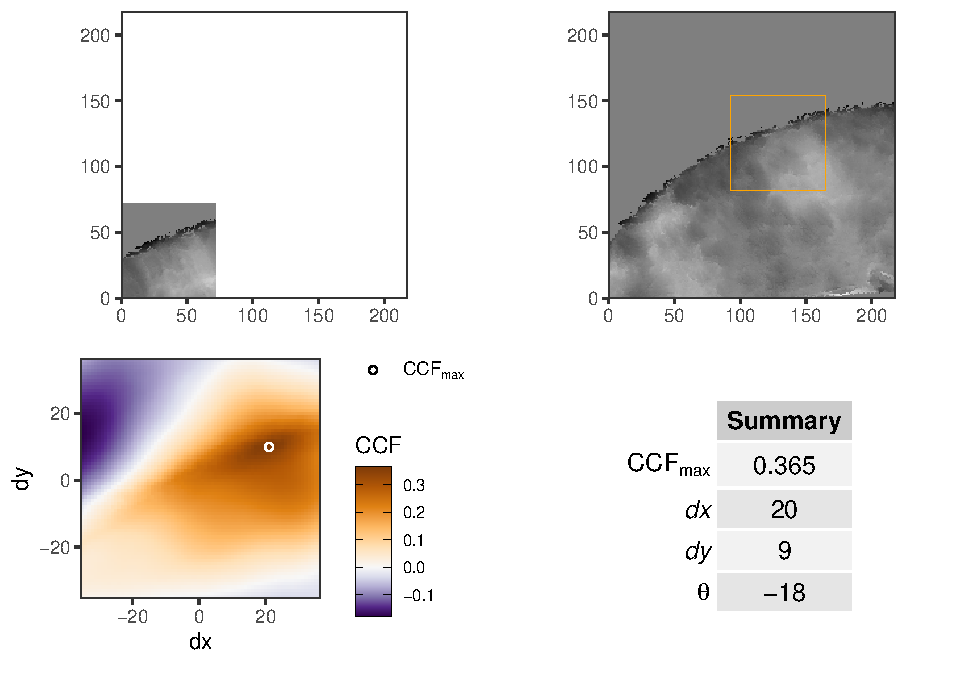
\includegraphics[width=\linewidth]{cmcR_files/figure-latex/unnamed-chunk-2-1} 

}

\caption{\label{fig:ccfMap_example} Example of a cross-correlation function "map" for a particular cell/region comparison}\label{fig:unnamed-chunk-2}
\end{figure}
\end{Schunk}

Using the estimated translation values at which the CCF\(_{\max}\)
occurs, we can calculate the pairwise-complete cross-correlation between
the cell and a cell-sized matrix extracted from the larger region where
missing values are not replaced. Think of this as punching-out the
matrix enclosed in the orange square shown in the top-right plot of
Figure \ref{fig:ccfMap_example}. This will be used as the high
CCF\(_{\max}\) estimate. This cell-based comparison procedure is
performed for each cell/region pair for various rotation values.

\hypertarget{the-congruent-matching-cells-method}{%
\subsection{The Congruent Matching Cells
method}\label{the-congruent-matching-cells-method}}

A particular cell/region pair is deemed ``highly similar'' if it passes
a collection of user-defined similarity criteria. The criteria are based
on the fact that a pair of matching cartridge case scans are not
necessarily aligned properly in their raw format. In particular, one
cartridge case scan needs to be rotated and translated to align
correctly the other. Let CCF\(_{\max}, dx, dy, \theta\) denote the
``true'' but unknown CCF, translation, and rotation values by which a
particular pair aligns the best. These unknown alignment parameters can
be estimated for each cell/region pair using the cell-based comparison
procedure discussed in section
\protect\hyperlink{comparisonProcedure}{3.1}. Let
CCF\(_{\max,i}, dx_i, dy_i, \theta_i\) denote the estimated alignment
parameter values for cell/region pair \(i\), \(i = 1,...,n\). For a
truly matching pair of cartridge cases, we would expect these alignment
parameter estimates to agree with each other across cell/region pairs;
at least up to some threshold. Conversely, we would expect the estimates
to vary randomly for a truly \emph{non}-matching pair. As such, the CMC
method details how to determine whether a consensus exists among the
estimated alignment parameter values across the cell/region pairs. The
initially proposed method by \citet{song_proposed_2013} as well as an
extension by \citet{tong_improved_2015} known as the High CMC method are
implemented in the \pkg{cmcR} package.

\hypertarget{initialMethod}{%
\subsubsection{The initially proposed method}\label{initialMethod}}

The method as originally proposed by \citet{song_proposed_2013}
considers only the alignment parameter estimates by which each
cell/region pair attains its CCF\(_{\max,i}\). Intuitively, this can be
thought of as only allowing each cell/region pair to ``vote'' for a
single set of alignment parameter values. It's reasonable to assume that
a consensus would exist amongst these values for a truly matching pair
of cartridge cases. Song proposes using the median of the
\(dx_i, dy_i, \theta_i\) values as a consensus, although others are
certainly plausible. Let
\(\overline{dx}, \overline{dy}, \overline{\theta}\) denote the
consensual alignment parameter values. To declare a particular
cell/region pair as ``conruent matching,'' Song requires that (1) the
pair's estimated alignment parameter values be within some threshold
distance of the consensual values and (2) the CCF\(_{\max}\) value is
greater than some threshold. That is, for thresholds
\(T_{dx}, T_{dy}, T_{\theta},T_{\text{CCF}}\), cell/region pair \(i\) is
declared a match if all of the following conditions hold:

\begin{enumerate}
\item $|dx_i - \overline{dx}| \leq T_{dx}$ \\
\item $|dy_i - \overline{dy}| \leq T_{dy}$ \\
\item $|\theta_i - \bar{\theta}| \leq T_{\theta}$ \\
\item CCF$_{\max,i} \geq T_{\text{CCF}}$.
\end{enumerate}

Song proposes using a minimum of 6 congruent matching cells to declare a
cartridge case pair a match, although this threshold is based on a
common threshold used in matching bullets via the striae left by a
firearm barrel. This has been shown in subsequent extensions to not
always be an effective threshold \citep{chen_convergence_2017}.

\hypertarget{highCMCMethod}{%
\subsubsection{The High CMC method}\label{highCMCMethod}}

Experimentation demonstrated that the assumption underlying the
initially proposed method, that the CCF\(_{\max,i}\) estimated alignment
parameter values would reach a consensus across all cell/region pairs,
does not always hold in general. In particular, if we only consider the
``top'' vote for each cell/region pair, then many pairs may vote far
away from the consensual value and thus would not be declared congruent
matching. However, \citet{tong_improved_2015} observe that such pairs
\emph{are} often highly similar at the consensual rotation value,
\(\overline{\theta}\). The extension they propose utilizes the behavior
of the estimated alignment parameter values more advantageously across
various rotation values than the initially proposed method.
Additionally, comparisons are performed in both ``directions'' so that
each cartridge case scan takes on the role of the scan that is
partitioned into a grid of cells.

\citet{tong_improved_2015} propose applying the translation and
CCF\(_{\max}\) CMC criteria discussed in section
\protect\hyperlink{initialMethod}{3.2.1} to the comparison results for
each rotation value. In doing so, a CMC count for each rotation can be
obtained. They identify a common behavior among known match cartridge
case pairs that the CMC counts often attain a mode around the rotation
value by which they align best. For known non-match pairs, the CMC
counts often vary randomly across rotation values. These phenomena are
illustrated in Figures \ref{fig:kmCMCPerTheta} and
\ref{fig:knmCMCPerTheta}. Figure \ref{fig:kmCMCPerTheta} shows the CMC
counts per rotation value in both directions for a known match pair of
cartridge case scans from \citet{fadul_empirical_nodate}. We can clearly
see a CMC mode around \(\theta = -21\) in one direction and \(21\) or
\(24\) in the other, which is to be expected for a known match pair.
Figure \ref{fig:knmCMCPerTheta}, on the other hand, shows the CMC counts
for a known non-match pair. We can see that no such CMC count mode is
achieved.

\citet{tong_improved_2015} introduce an additional criterion to identify
a mode in the CMC per \(\theta\) counts. Namely, they introduce a
``high'' CMC threshold defined to be CMC\(_{\text{high}} =\)
CMC\(_{\max} - \tau\) for some constant \(\tau\) (they choose
\(\tau = 1\)) where CMC\(_{\max}\) is the maximum CMC count attained
across all rotation values considered. In the example shown in Figure
\ref{fig:kmCMCPerTheta}, CMC\(_{\max} = 17\) in one direction and 15 in
the other. They propose finding the range of rotation values with
associated CMC count greater than or equal to CMC\(_{\text{high}}\). If
this range is greater than the threshold \(T_\theta\), then there is
evidence to suggest that a CMC count mode does not exist and the
cartridge case pair is not a match. The CMC\(_{\text{high}}\) thresholds
are shown as horizontal dashed lines in Figures \ref{fig:kmCMCPerTheta}
and \ref{fig:knmCMCPerTheta}. We can see in Figure
\ref{fig:kmCMCPerTheta} that the only \(\theta\) values with associated
CMC counts greater than or equal to CMC\(_{\text{high}}\) are adjacent.
This particular cartridge case pair would ``pass'' the high CMC
criterion. The pair shown in Figure \ref{fig:knmCMCPerTheta} elicit
considerably more diffuse \(\theta\) values with associated CMC count
great than or equal to CMC\(_{\text{high}}\) and thus would not pass the
high CMC criterion.

\begin{Schunk}
\begin{figure}[h]

{\centering 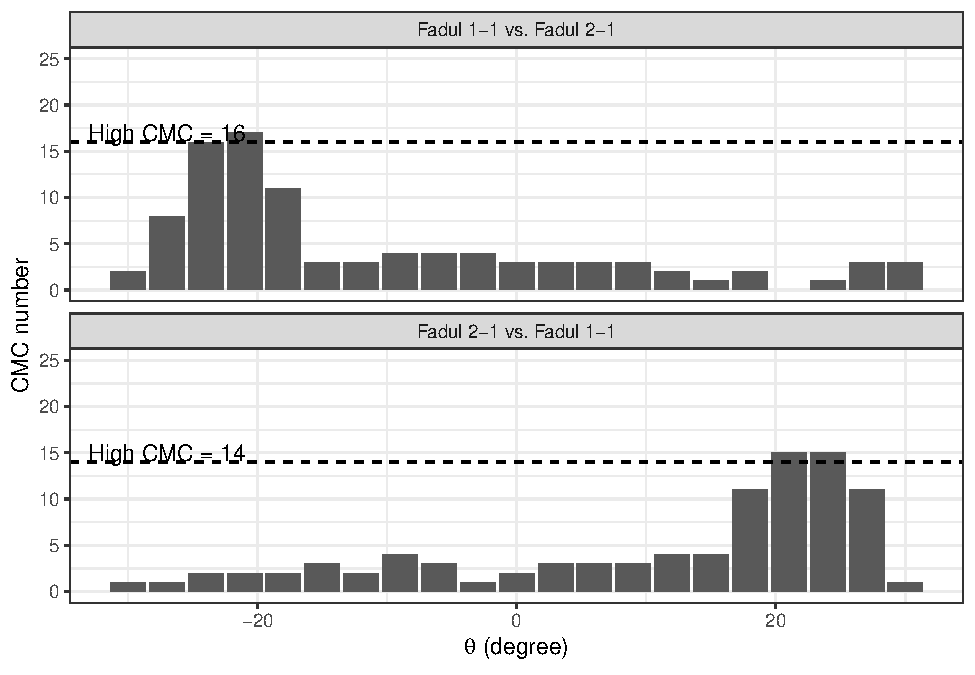
\includegraphics[width=.7\textwidth]{cmcR_files/figure-latex/unnamed-chunk-3-1} 

}

\caption{\label{fig:kmCMCPerTheta} CMC count per rotation ($\theta$) values in both directions for a KM cartridge case pair}\label{fig:unnamed-chunk-3}
\end{figure}
\end{Schunk}

\begin{Schunk}
\begin{figure}[h]

{\centering 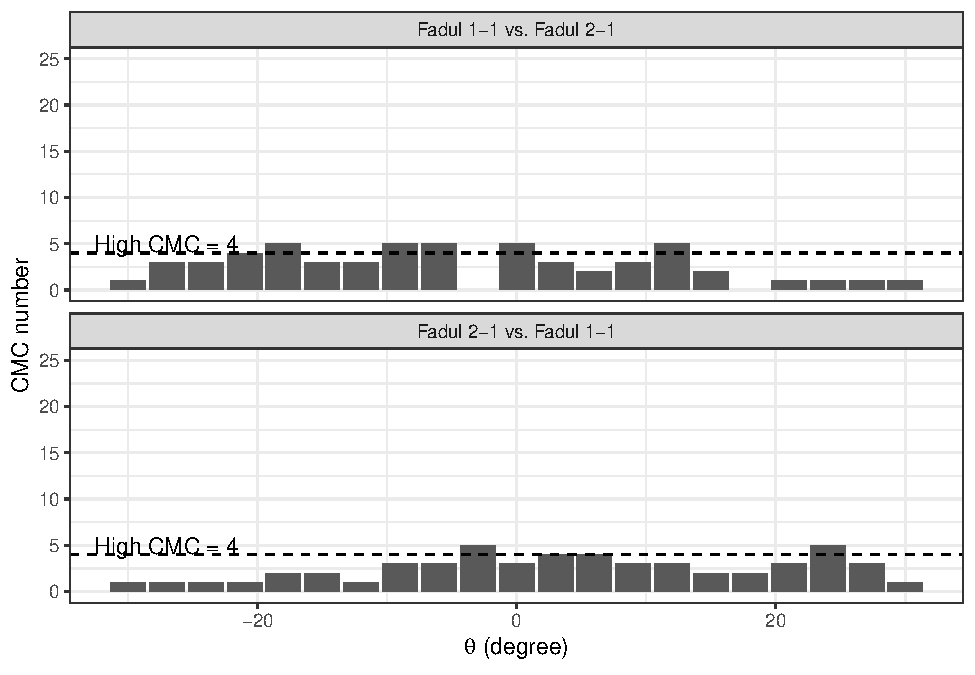
\includegraphics[width=.7\textwidth]{cmcR_files/figure-latex/unnamed-chunk-5-1} 

}

\caption{\label{fig:knmCMCPerTheta} CMC count per rotation ($\theta$) values in both directions for a KNM cartridge case pair}\label{fig:unnamed-chunk-5}
\end{figure}
\end{Schunk}

Cartridge case pairs that do not pass the high CMC criterion are
assigned the CMC count under the initially proposed method. Pairs that
do pass the criterion are assigned all CMCs in and within \(T_\theta\)
of the identified CMC count mode in both directions (excluding
replicates). Among other considerations, \citet{tong_improved_2015} do
not indicate how to deal with adjacent CMC count ties (as is the case in
the Fadul 1-2 vs.~Fadul 1-1 direction in Figure \ref{fig:kmCMCPerTheta})
nor situtations in which a CMC count mode is identified in one direction
but not the other. This, again, illustates how a qualitative description
of a method often fails to cover critical details. While individually
small in scope, leaving such details ambiguous can quickly compound how
difficult it is to effectively reproduce results.

\hypertarget{the-package}{%
\subsection{\texorpdfstring{The \pkg{cmcR}
package}{The  package}}\label{the-package}}

This section will highlight the \pkg{cmcR} package's functionality by
walking through a possible use case. Many of the functions in this
package provide the user with a variety of processing options with which
they can experiment. This is due to the fact that processing techniques
differ considerably among authors or are not discussed in great detail.

\hypertarget{pre-processing-procedures}{%
\subsubsection{Pre-processing
procedures}\label{pre-processing-procedures}}

Studies in which cartridge cases are matched by forensic examiners often
involve giving examiners a set of known matches and asking them to
classify additional matches from a collection of unknown source scans.
For brevity, we will consider a comparison between two cartridge cases.
This particular pair of scans, as well as many other cartridge case
scans, are openly available from the NIST Ballistics and Toolmarks
Research Database. Figure \ref{fig:processedScans} shows the pair of
scans after performing the necessary pre-processing procedures. Note
that the color scheme has been scaled by quantiles to visually highlight
regions of the cartridge case scan containing strong breech face
impression ``signal.''

\begin{Schunk}
\begin{figure}[htbp]

{\centering 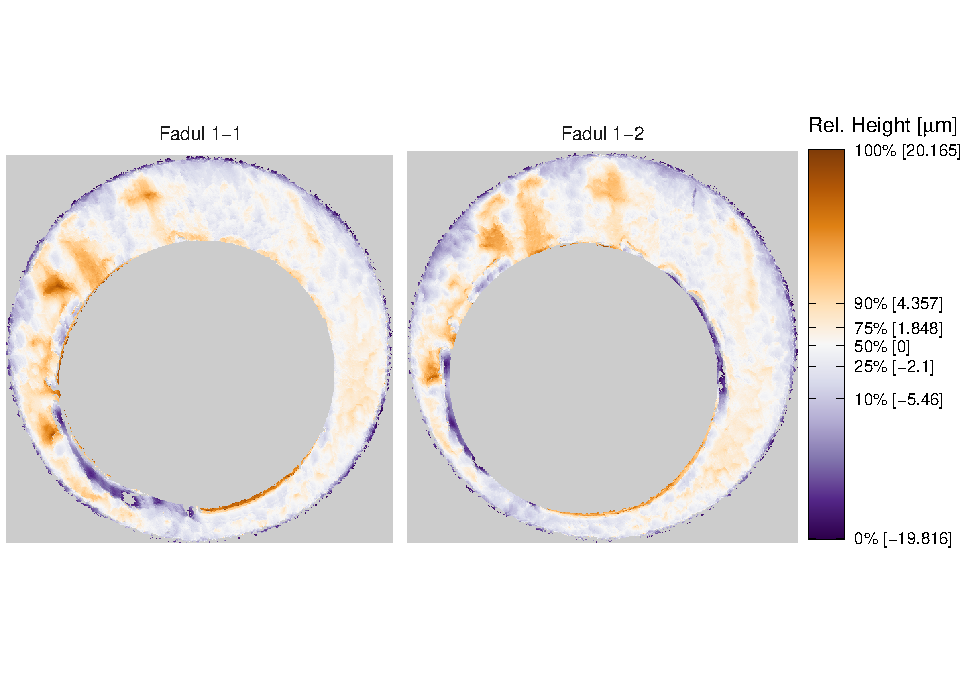
\includegraphics[width=1.2\textwidth,trim={0 2.5cm 0 2cm}]{cmcR_files/figure-latex/unnamed-chunk-6-1} 

}

\caption{\label{fig:processedScans} A known match pair of processed cartridge case scans}\label{fig:unnamed-chunk-6}
\end{figure}
\end{Schunk}

The family of functions in the \pkg{cmcR} package beginning with
\code{preProcess\_} can be used to perform the necessary pre-processing
steps for a pair of cartridge case scans to be comparable using the
cell-based comparison procedure outlined in section
\protect\hyperlink{comparisonProcedure}{3.1}. The implementation of many
of these pre-processing procedures is inspired largely by
\citet{tai_fully_2018} who detail a fully-automatic procedure for
processing cartridge case 2D images as opposed to 3D scans. The
functions available include:

\begin{enumerate}
\item \code{preProcess\_ransac}: estimates the height value of the breech face impressions in a scan using the Random Sample Consensus (RANSAC) robust, iterative plane-fitting algorithm \citep{ransac}.

\item \code{preProcess\_levelBF}: extracts the observations containing breech face impressions from the scan using the estimated height value obtained from \code{preProcess\_levelBF}.

\item \code{preProcess\_cropWS}: removes rows/columns containing mostly if not all \code{NA} values from the surface matrix on the exterior of breech face impressions.

\item \code{preProcess\_removeFPCircle}: detects and removes observations within the firing pin impression circle using the Hough Transform circle detection algorithm \citep{hough}.

\item \code{preProcess\_gaussFilter}: applies a low-pass, high-pass, or band-pass Gaussian filter to the breech face impressions to reduce the effects of high frequency noise, low frequency global structure, or both, respectively.
\end{enumerate}

See the \pkg{cmcR} package documentation for more information about
these functions.

For computational purposes it is common the CMC literature to
down-sample a surface matrix prior to performing the cell-based
comparison procedure. The \code{sample\_x3p} function from the
\pkg{x3ptools} package can be used used to sample every \(m\)th
row/column of a surface matrix. The
\code{selectBFImpression\_sample\_x3p} performs all of these
pre-processing procedures in a single call. The code to produce the
first surface matrix shown in Figure \ref{fig:processedScans} is given
by the following example. Note that the RANSAC method relies on randomly
selecting points within the surface matrix, so a seed needs to be set
for reproducibility.

\begin{Schunk}
\begin{Sinput}
library(cmcR)
library(x3ptools)
library(magrittr)
set.seed(4132020)

nrbtd_url <- "https://tsapps.nist.gov/NRBTD/Studies/CartridgeMeasurement/"

fadul1.1_id <- "DownloadMeasurement/2d9cc51f-6f66-40a0-973a-a9292dbee36d"
fadul1.2_id <- "DownloadMeasurement/cb296c98-39f5-46eb-abff-320a2f5568e8"

fadul1.1 <- selectBFImpression_sample_x3p(x3p_path = paste0(nrbtd_url,fadul1.1_id),
                                          ransacInlierThresh = 1e-5, #1 micron
                                          ransacIters = 150,
                                          croppingThresh = 1,
                                          m = 2, #sample_x3p down-sample rate
                                          gaussFilterWavelength = c(16,250),
                                          gaussFilterType = "bp") #band-pass filter
\end{Sinput}
\end{Schunk}

\subsection{Implementation of cell-based comparison procedure}

The cell-based comparison procedure outlined in section
\protect\hyperlink{comparisonProcedure}{3.1} is implemented in the
\code{cellCCF\_bothDirections} function. In particular, the procedure is
performed twice so that both cartridge case scans take on the role of
the scan that is partitioned into a grid of cells. This is necessary to
apply the High CMC logic discussed in section
\protect\hyperlink{highCMCMethod}{3.2.2}. Continuing with the current
use case example, the code to perform this procedure on \code{fadul1.1}
and \code{fadul1.2} is given by the following example.

\begin{Schunk}
\begin{Sinput}
kmComparison <- cellCCF_bothDirections(x3p1 = fadul1.1,
                                       x3p2 = fadul1.2,
                                       thetas = seq(-30,30,by = 3),
                                       cellNumHoriz = 8,
                                       cellNumVert = cellNumHoriz,
                                       minObservedProp = .1)
\end{Sinput}
\end{Schunk}

The first few rows of results from the comparison between
\code{fadul1.1} and \code{fadul1.2} in which \code{fadul1.1} was divided
into a grid of cells and \code{fadul1.2} was rotated by 3 degrees is
given below. Although a grid of \(8 \times 8\) cells were used, there
were only 43 cell/region pairs that contained a sufficient proportion of
non-missing values (10\% in this example). Recall that the features used
in the CMC method are the CCF\(_{\max}\) values (\code{ccf} column) and
estimated alignment parameter values (\code{dx}, \code{dy}, and
\code{theta} columns).

\begin{Schunk}
\begin{Sinput}
kmComparison$comparison_1to2$ccfResults$`3` %>%
  head()
\end{Sinput}
\end{Schunk}

\begin{Schunk}
\begin{table}[!h]

\caption{\label{tab:unnamed-chunk-10}\label{tab:cellCCF} Example of output from \code{cellCCF} function}
\centering
\begin{tabular}[t]{r|l|r|r|r|r|r}
\hline
cellNum & cellID & ccf & fft.ccf & dx & dy & theta\\
\hline
2 & y = 1 - 73, x = 74 - 145 & 0.7762319 & 0.2108462 & 34 & -30 & 3\\
\hline
3 & y = 1 - 73, x = 146 - 217 & 0.1006877 & 0.1145874 & 29 & 22 & 3\\
\hline
4 & y = 1 - 73, x = 218 - 289 & 0.1863672 & 0.1030728 & -32 & -16 & 3\\
\hline
5 & y = 1 - 73, x = 290 - 362 & 0.8004083 & 0.3658809 & 5 & 4 & 3\\
\hline
6 & y = 1 - 73, x = 363 - 434 & 0.7036884 & 0.2353348 & 22 & 10 & 3\\
\hline
7 & y = 1 - 73, x = 435 - 506 & 0.7965972 & 0.1407746 & -25 & -18 & 3\\
\hline
\end{tabular}
\end{table}

\end{Schunk}

\hypertarget{congruent-matching-cells-logic}{%
\subsection{Congruent Matching Cells
logic}\label{congruent-matching-cells-logic}}

\begin{Schunk}
\begin{Sinput}
kmCMC <- cmcR::cmcFilter_improved(kmComparison,
                                  ccf_thresh = .5,
                                  dx_thresh = 20,
                                  theta_thresh = 6)

cmcPlots <- cmcR::cmcPlot(fadul1.1$x3p,
                          fadul1.2$x3p,
                          cellCCF_bothDirections_output = kmComparison,
                          cmcFilter_improved_output = kmCMC,
                          x3pNames = c("Fadul 1-1","Fadul 1-2")) 

cmcPlots$initialCMC
\end{Sinput}
\end{Schunk}

\begin{Schunk}
\begin{figure}[htbp]

{\centering 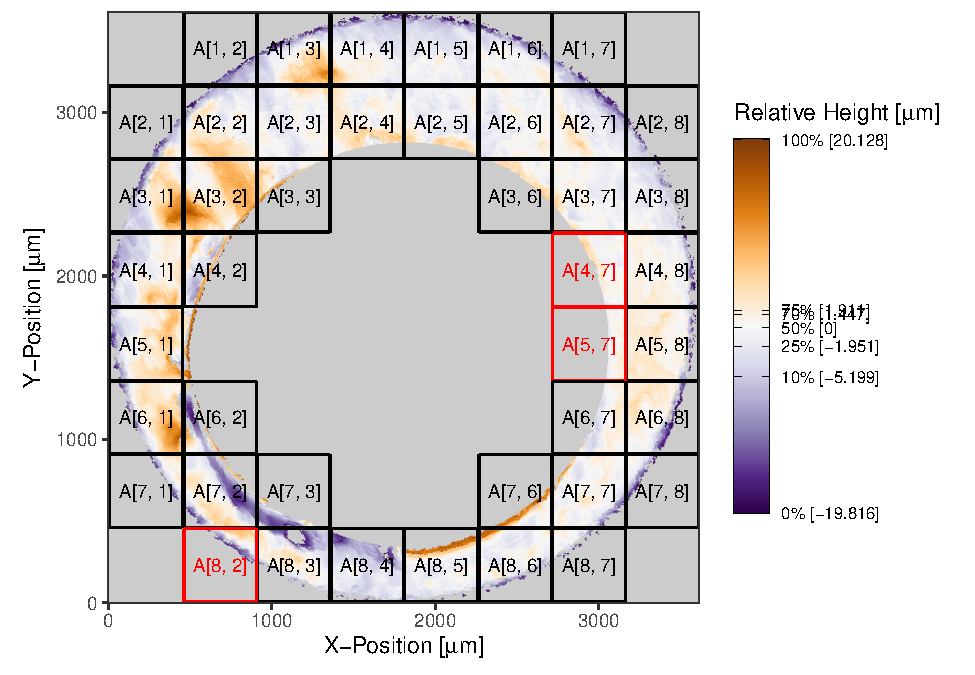
\includegraphics[width=1.2\textwidth,trim={0 2.5cm 0 2cm}]{cmcR_files/figure-latex/unnamed-chunk-12-1} 

}

\caption{\label{fig:initialCMCPlot} CMC results from a known match comparison under the initially proposed method}\label{fig:unnamed-chunk-12}
\end{figure}
\end{Schunk}

The CMCs determined under the High CMC method (i.e., the ``high'' CMCs)
are show below. We can see that 40 out of the

\begin{Schunk}
\begin{Sinput}
cmcPlots$highCMC
\end{Sinput}
\end{Schunk}

\begin{Schunk}
\begin{figure}[htbp]

{\centering 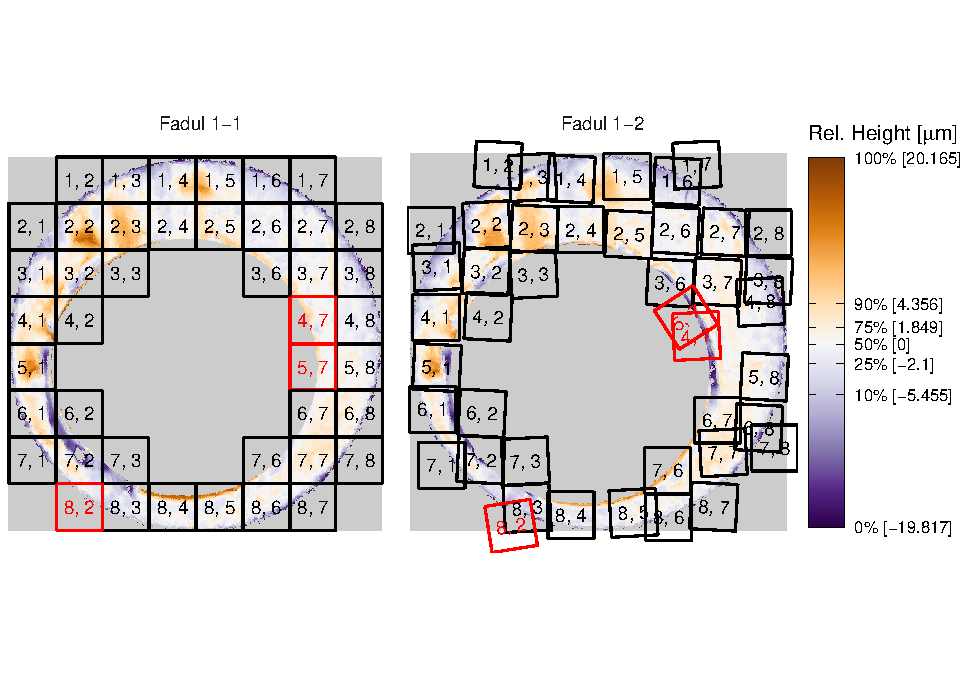
\includegraphics[width=1.2\textwidth,trim={0 2.5cm 0 2cm}]{cmcR_files/figure-latex/unnamed-chunk-14-1} 

}

\caption{\label{fig:highCMCPlot} CMC results from a known match comparison under the High CMC method}\label{fig:unnamed-chunk-14}
\end{figure}
\end{Schunk}

\bibliography{RJreferences}


\address{%
Joseph Zemmels\\
Iowa State University Department of Statistics\\
2438 Osborn Dr\\ Ames, IA 50011\\
}
\href{mailto:jzemmels@iastate.edu}{\nolinkurl{jzemmels@iastate.edu}}

\address{%
Heike Hofmann\\
Iowa State University Department of Statistics\\
2438 Osborn Dr\\ Ames, IA 50011\\
}
\href{mailto:hofmann@iastate.edu}{\nolinkurl{hofmann@iastate.edu}}

\address{%
Susan VanderPlas\\
University of Nebraska - Lincoln Department of Statistics\\
340 Hardin Hall North Wing\\ Lincoln, NE 68583\\
}
\href{mailto:susan.vanderplas@iastate.edu}{\nolinkurl{susan.vanderplas@iastate.edu}}

